% Created by tikzDevice version 0.10.1 on 2016-08-19 15:25:34
% !TEX encoding = UTF-8 Unicode
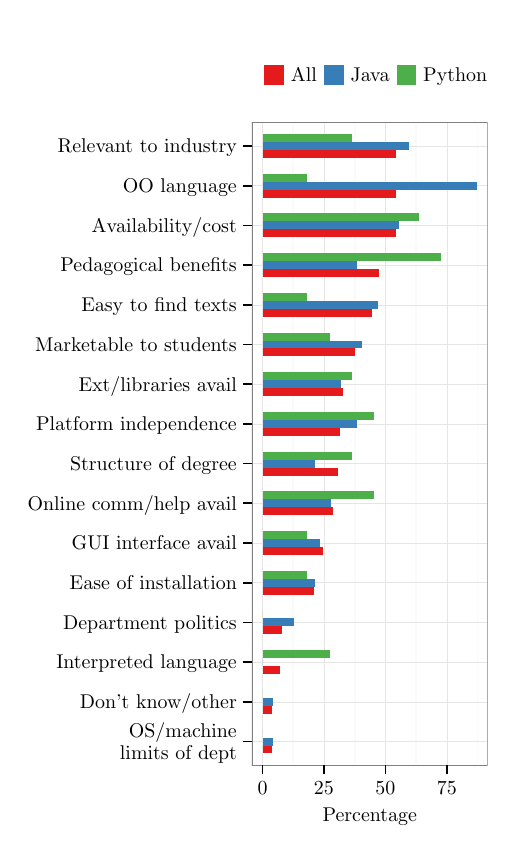
\begin{tikzpicture}[x=1pt,y=1pt]
\definecolor{fillColor}{RGB}{255,255,255}
\path[use as bounding box,fill=fillColor,fill opacity=0.00] (0,0) rectangle (166.22,289.08);
\begin{scope}
\path[clip] (  0.00,  0.00) rectangle (166.22,289.08);
\definecolor{drawColor}{RGB}{255,255,255}
\definecolor{fillColor}{RGB}{255,255,255}

\path[draw=drawColor,line width= 0.6pt,line join=round,line cap=round,fill=fillColor] (  0.00,  0.00) rectangle (166.22,289.08);
\end{scope}
\begin{scope}
\path[clip] ( 80.98, 22.52) rectangle (166.22,254.94);
\definecolor{fillColor}{RGB}{255,255,255}

\path[fill=fillColor] ( 80.98, 22.52) rectangle (166.22,254.94);
\definecolor{drawColor}{gray}{0.98}

\path[draw=drawColor,line width= 0.6pt,line join=round] ( 95.96, 22.52) --
	( 95.96,254.94);

\path[draw=drawColor,line width= 0.6pt,line join=round] (118.17, 22.52) --
	(118.17,254.94);

\path[draw=drawColor,line width= 0.6pt,line join=round] (140.38, 22.52) --
	(140.38,254.94);

\path[draw=drawColor,line width= 0.6pt,line join=round] (162.59, 22.52) --
	(162.59,254.94);
\definecolor{drawColor}{gray}{0.90}

\path[draw=drawColor,line width= 0.2pt,line join=round] ( 80.98, 31.13) --
	(166.22, 31.13);

\path[draw=drawColor,line width= 0.2pt,line join=round] ( 80.98, 45.47) --
	(166.22, 45.47);

\path[draw=drawColor,line width= 0.2pt,line join=round] ( 80.98, 59.82) --
	(166.22, 59.82);

\path[draw=drawColor,line width= 0.2pt,line join=round] ( 80.98, 74.17) --
	(166.22, 74.17);

\path[draw=drawColor,line width= 0.2pt,line join=round] ( 80.98, 88.51) --
	(166.22, 88.51);

\path[draw=drawColor,line width= 0.2pt,line join=round] ( 80.98,102.86) --
	(166.22,102.86);

\path[draw=drawColor,line width= 0.2pt,line join=round] ( 80.98,117.21) --
	(166.22,117.21);

\path[draw=drawColor,line width= 0.2pt,line join=round] ( 80.98,131.55) --
	(166.22,131.55);

\path[draw=drawColor,line width= 0.2pt,line join=round] ( 80.98,145.90) --
	(166.22,145.90);

\path[draw=drawColor,line width= 0.2pt,line join=round] ( 80.98,160.25) --
	(166.22,160.25);

\path[draw=drawColor,line width= 0.2pt,line join=round] ( 80.98,174.59) --
	(166.22,174.59);

\path[draw=drawColor,line width= 0.2pt,line join=round] ( 80.98,188.94) --
	(166.22,188.94);

\path[draw=drawColor,line width= 0.2pt,line join=round] ( 80.98,203.29) --
	(166.22,203.29);

\path[draw=drawColor,line width= 0.2pt,line join=round] ( 80.98,217.63) --
	(166.22,217.63);

\path[draw=drawColor,line width= 0.2pt,line join=round] ( 80.98,231.98) --
	(166.22,231.98);

\path[draw=drawColor,line width= 0.2pt,line join=round] ( 80.98,246.33) --
	(166.22,246.33);

\path[draw=drawColor,line width= 0.2pt,line join=round] ( 84.86, 22.52) --
	( 84.86,254.94);

\path[draw=drawColor,line width= 0.2pt,line join=round] (107.06, 22.52) --
	(107.06,254.94);

\path[draw=drawColor,line width= 0.2pt,line join=round] (129.27, 22.52) --
	(129.27,254.94);

\path[draw=drawColor,line width= 0.2pt,line join=round] (151.48, 22.52) --
	(151.48,254.94);
\definecolor{fillColor}{RGB}{228,26,28}

\path[fill=fillColor] ( 84.86, 26.82) rectangle ( 88.37, 29.69);
\definecolor{fillColor}{RGB}{55,126,184}

\path[fill=fillColor] ( 84.86, 29.69) rectangle ( 88.64, 32.56);
\definecolor{fillColor}{RGB}{77,175,74}

\path[fill=fillColor] ( 84.86, 32.56) rectangle ( 84.86, 35.43);
\definecolor{fillColor}{RGB}{228,26,28}

\path[fill=fillColor] ( 84.86, 41.17) rectangle ( 88.37, 44.04);
\definecolor{fillColor}{RGB}{55,126,184}

\path[fill=fillColor] ( 84.86, 44.04) rectangle ( 88.64, 46.91);
\definecolor{fillColor}{RGB}{77,175,74}

\path[fill=fillColor] ( 84.86, 46.91) rectangle ( 84.86, 49.78);
\definecolor{fillColor}{RGB}{228,26,28}

\path[fill=fillColor] ( 84.86, 55.52) rectangle ( 91.01, 58.38);
\definecolor{fillColor}{RGB}{55,126,184}

\path[fill=fillColor] ( 84.86, 58.38) rectangle ( 84.86, 61.25);
\definecolor{fillColor}{RGB}{77,175,74}

\path[fill=fillColor] ( 84.86, 61.25) rectangle (109.08, 64.12);
\definecolor{fillColor}{RGB}{228,26,28}

\path[fill=fillColor] ( 84.86, 69.86) rectangle ( 91.89, 72.73);
\definecolor{fillColor}{RGB}{55,126,184}

\path[fill=fillColor] ( 84.86, 72.73) rectangle ( 96.20, 75.60);
\definecolor{fillColor}{RGB}{77,175,74}

\path[fill=fillColor] ( 84.86, 75.60) rectangle ( 84.86, 78.47);
\definecolor{fillColor}{RGB}{228,26,28}

\path[fill=fillColor] ( 84.86, 84.21) rectangle (103.32, 87.08);
\definecolor{fillColor}{RGB}{55,126,184}

\path[fill=fillColor] ( 84.86, 87.08) rectangle (103.76, 89.95);
\definecolor{fillColor}{RGB}{77,175,74}

\path[fill=fillColor] ( 84.86, 89.95) rectangle (101.01, 92.82);
\definecolor{fillColor}{RGB}{228,26,28}

\path[fill=fillColor] ( 84.86, 98.56) rectangle (106.84,101.43);
\definecolor{fillColor}{RGB}{55,126,184}

\path[fill=fillColor] ( 84.86,101.43) rectangle (105.64,104.29);
\definecolor{fillColor}{RGB}{77,175,74}

\path[fill=fillColor] ( 84.86,104.29) rectangle (101.01,107.16);
\definecolor{fillColor}{RGB}{228,26,28}

\path[fill=fillColor] ( 84.86,112.90) rectangle (110.36,115.77);
\definecolor{fillColor}{RGB}{55,126,184}

\path[fill=fillColor] ( 84.86,115.77) rectangle (109.43,118.64);
\definecolor{fillColor}{RGB}{77,175,74}

\path[fill=fillColor] ( 84.86,118.64) rectangle (125.23,121.51);
\definecolor{fillColor}{RGB}{228,26,28}

\path[fill=fillColor] ( 84.86,127.25) rectangle (112.12,130.12);
\definecolor{fillColor}{RGB}{55,126,184}

\path[fill=fillColor] ( 84.86,130.12) rectangle (103.76,132.99);
\definecolor{fillColor}{RGB}{77,175,74}

\path[fill=fillColor] ( 84.86,132.99) rectangle (117.16,135.86);
\definecolor{fillColor}{RGB}{228,26,28}

\path[fill=fillColor] ( 84.86,141.60) rectangle (113.00,144.47);
\definecolor{fillColor}{RGB}{55,126,184}

\path[fill=fillColor] ( 84.86,144.47) rectangle (118.88,147.34);
\definecolor{fillColor}{RGB}{77,175,74}

\path[fill=fillColor] ( 84.86,147.34) rectangle (125.23,150.20);
\definecolor{fillColor}{RGB}{228,26,28}

\path[fill=fillColor] ( 84.86,155.94) rectangle (113.88,158.81);
\definecolor{fillColor}{RGB}{55,126,184}

\path[fill=fillColor] ( 84.86,158.81) rectangle (113.20,161.68);
\definecolor{fillColor}{RGB}{77,175,74}

\path[fill=fillColor] ( 84.86,161.68) rectangle (117.16,164.55);
\definecolor{fillColor}{RGB}{228,26,28}

\path[fill=fillColor] ( 84.86,170.29) rectangle (118.28,173.16);
\definecolor{fillColor}{RGB}{55,126,184}

\path[fill=fillColor] ( 84.86,173.16) rectangle (120.77,176.03);
\definecolor{fillColor}{RGB}{77,175,74}

\path[fill=fillColor] ( 84.86,176.03) rectangle (109.08,178.90);
\definecolor{fillColor}{RGB}{228,26,28}

\path[fill=fillColor] ( 84.86,184.64) rectangle (124.43,187.51);
\definecolor{fillColor}{RGB}{55,126,184}

\path[fill=fillColor] ( 84.86,187.51) rectangle (126.44,190.38);
\definecolor{fillColor}{RGB}{77,175,74}

\path[fill=fillColor] ( 84.86,190.38) rectangle (101.01,193.25);
\definecolor{fillColor}{RGB}{228,26,28}

\path[fill=fillColor] ( 84.86,198.98) rectangle (127.07,201.85);
\definecolor{fillColor}{RGB}{55,126,184}

\path[fill=fillColor] ( 84.86,201.85) rectangle (118.88,204.72);
\definecolor{fillColor}{RGB}{77,175,74}

\path[fill=fillColor] ( 84.86,204.72) rectangle (149.47,207.59);
\definecolor{fillColor}{RGB}{228,26,28}

\path[fill=fillColor] ( 84.86,213.33) rectangle (133.24,216.20);
\definecolor{fillColor}{RGB}{55,126,184}

\path[fill=fillColor] ( 84.86,216.20) rectangle (134.00,219.07);
\definecolor{fillColor}{RGB}{77,175,74}

\path[fill=fillColor] ( 84.86,219.07) rectangle (141.39,221.94);
\definecolor{fillColor}{RGB}{228,26,28}

\path[fill=fillColor] ( 84.86,227.68) rectangle (133.24,230.55);
\definecolor{fillColor}{RGB}{55,126,184}

\path[fill=fillColor] ( 84.86,230.55) rectangle (162.35,233.42);
\definecolor{fillColor}{RGB}{77,175,74}

\path[fill=fillColor] ( 84.86,233.42) rectangle (101.01,236.29);
\definecolor{fillColor}{RGB}{228,26,28}

\path[fill=fillColor] ( 84.86,242.02) rectangle (133.24,244.89);
\definecolor{fillColor}{RGB}{55,126,184}

\path[fill=fillColor] ( 84.86,244.89) rectangle (137.77,247.76);
\definecolor{fillColor}{RGB}{77,175,74}

\path[fill=fillColor] ( 84.86,247.76) rectangle (117.16,250.63);
\definecolor{drawColor}{gray}{0.50}

\path[draw=drawColor,line width= 0.6pt,line join=round,line cap=round] ( 80.98, 22.52) rectangle (166.22,254.94);
\end{scope}
\begin{scope}
\path[clip] (  0.00,  0.00) rectangle (166.22,289.08);
\definecolor{drawColor}{RGB}{0,0,0}

\node[text=drawColor,anchor=base east,inner sep=0pt, outer sep=0pt, scale=  0.72] at ( 75.58, 32.53) {OS/machine};

\node[text=drawColor,anchor=base east,inner sep=0pt, outer sep=0pt, scale=  0.72] at ( 75.58, 24.76) {limits of dept};

\node[text=drawColor,anchor=base east,inner sep=0pt, outer sep=0pt, scale=  0.72] at ( 75.58, 42.99) {Don't know/other};

\node[text=drawColor,anchor=base east,inner sep=0pt, outer sep=0pt, scale=  0.72] at ( 75.58, 57.34) {Interpreted language};

\node[text=drawColor,anchor=base east,inner sep=0pt, outer sep=0pt, scale=  0.72] at ( 75.58, 71.69) {Department politics};

\node[text=drawColor,anchor=base east,inner sep=0pt, outer sep=0pt, scale=  0.72] at ( 75.58, 86.03) {Ease of installation};

\node[text=drawColor,anchor=base east,inner sep=0pt, outer sep=0pt, scale=  0.72] at ( 75.58,100.38) {GUI interface avail};

\node[text=drawColor,anchor=base east,inner sep=0pt, outer sep=0pt, scale=  0.72] at ( 75.58,114.73) {Online comm/help avail};

\node[text=drawColor,anchor=base east,inner sep=0pt, outer sep=0pt, scale=  0.72] at ( 75.58,129.07) {Structure of degree};

\node[text=drawColor,anchor=base east,inner sep=0pt, outer sep=0pt, scale=  0.72] at ( 75.58,143.42) {Platform independence};

\node[text=drawColor,anchor=base east,inner sep=0pt, outer sep=0pt, scale=  0.72] at ( 75.58,157.77) {Ext/libraries avail};

\node[text=drawColor,anchor=base east,inner sep=0pt, outer sep=0pt, scale=  0.72] at ( 75.58,172.11) {Marketable to students};

\node[text=drawColor,anchor=base east,inner sep=0pt, outer sep=0pt, scale=  0.72] at ( 75.58,186.46) {Easy to find texts};

\node[text=drawColor,anchor=base east,inner sep=0pt, outer sep=0pt, scale=  0.72] at ( 75.58,200.81) {Pedagogical benefits};

\node[text=drawColor,anchor=base east,inner sep=0pt, outer sep=0pt, scale=  0.72] at ( 75.58,215.16) {Availability/cost};

\node[text=drawColor,anchor=base east,inner sep=0pt, outer sep=0pt, scale=  0.72] at ( 75.58,229.50) {OO language};

\node[text=drawColor,anchor=base east,inner sep=0pt, outer sep=0pt, scale=  0.72] at ( 75.58,243.85) {Relevant to industry};
\end{scope}
\begin{scope}
\path[clip] (  0.00,  0.00) rectangle (166.22,289.08);
\definecolor{drawColor}{RGB}{0,0,0}

\path[draw=drawColor,line width= 0.6pt,line join=round] ( 77.98, 31.13) --
	( 80.98, 31.13);

\path[draw=drawColor,line width= 0.6pt,line join=round] ( 77.98, 45.47) --
	( 80.98, 45.47);

\path[draw=drawColor,line width= 0.6pt,line join=round] ( 77.98, 59.82) --
	( 80.98, 59.82);

\path[draw=drawColor,line width= 0.6pt,line join=round] ( 77.98, 74.17) --
	( 80.98, 74.17);

\path[draw=drawColor,line width= 0.6pt,line join=round] ( 77.98, 88.51) --
	( 80.98, 88.51);

\path[draw=drawColor,line width= 0.6pt,line join=round] ( 77.98,102.86) --
	( 80.98,102.86);

\path[draw=drawColor,line width= 0.6pt,line join=round] ( 77.98,117.21) --
	( 80.98,117.21);

\path[draw=drawColor,line width= 0.6pt,line join=round] ( 77.98,131.55) --
	( 80.98,131.55);

\path[draw=drawColor,line width= 0.6pt,line join=round] ( 77.98,145.90) --
	( 80.98,145.90);

\path[draw=drawColor,line width= 0.6pt,line join=round] ( 77.98,160.25) --
	( 80.98,160.25);

\path[draw=drawColor,line width= 0.6pt,line join=round] ( 77.98,174.59) --
	( 80.98,174.59);

\path[draw=drawColor,line width= 0.6pt,line join=round] ( 77.98,188.94) --
	( 80.98,188.94);

\path[draw=drawColor,line width= 0.6pt,line join=round] ( 77.98,203.29) --
	( 80.98,203.29);

\path[draw=drawColor,line width= 0.6pt,line join=round] ( 77.98,217.63) --
	( 80.98,217.63);

\path[draw=drawColor,line width= 0.6pt,line join=round] ( 77.98,231.98) --
	( 80.98,231.98);

\path[draw=drawColor,line width= 0.6pt,line join=round] ( 77.98,246.33) --
	( 80.98,246.33);
\end{scope}
\begin{scope}
\path[clip] (  0.00,  0.00) rectangle (166.22,289.08);
\definecolor{drawColor}{RGB}{0,0,0}

\path[draw=drawColor,line width= 0.6pt,line join=round] ( 84.86, 19.52) --
	( 84.86, 22.52);

\path[draw=drawColor,line width= 0.6pt,line join=round] (107.06, 19.52) --
	(107.06, 22.52);

\path[draw=drawColor,line width= 0.6pt,line join=round] (129.27, 19.52) --
	(129.27, 22.52);

\path[draw=drawColor,line width= 0.6pt,line join=round] (151.48, 19.52) --
	(151.48, 22.52);
\end{scope}
\begin{scope}
\path[clip] (  0.00,  0.00) rectangle (166.22,289.08);
\definecolor{drawColor}{RGB}{0,0,0}

\node[text=drawColor,anchor=base,inner sep=0pt, outer sep=0pt, scale=  0.72] at ( 84.86, 12.16) {0};

\node[text=drawColor,anchor=base,inner sep=0pt, outer sep=0pt, scale=  0.72] at (107.06, 12.16) {25};

\node[text=drawColor,anchor=base,inner sep=0pt, outer sep=0pt, scale=  0.72] at (129.27, 12.16) {50};

\node[text=drawColor,anchor=base,inner sep=0pt, outer sep=0pt, scale=  0.72] at (151.48, 12.16) {75};
\end{scope}
\begin{scope}
\path[clip] (  0.00,  0.00) rectangle (166.22,289.08);
\definecolor{drawColor}{RGB}{0,0,0}

\node[text=drawColor,anchor=base,inner sep=0pt, outer sep=0pt, scale=  0.72] at (123.60,  2.40) {Percentage};
\end{scope}
\begin{scope}
\path[clip] (  0.00,  0.00) rectangle (166.22,289.08);
\definecolor{fillColor}{RGB}{255,255,255}

\path[fill=fillColor] ( 76.91,263.47) rectangle (170.29,280.54);
\end{scope}
\begin{scope}
\path[clip] (  0.00,  0.00) rectangle (166.22,289.08);
\definecolor{fillColor}{RGB}{228,26,28}

\path[fill=fillColor] ( 85.50,268.45) rectangle ( 92.62,275.56);
\end{scope}
\begin{scope}
\path[clip] (  0.00,  0.00) rectangle (166.22,289.08);
\definecolor{fillColor}{RGB}{55,126,184}

\path[fill=fillColor] (107.05,268.45) rectangle (114.16,275.56);
\end{scope}
\begin{scope}
\path[clip] (  0.00,  0.00) rectangle (166.22,289.08);
\definecolor{fillColor}{RGB}{77,175,74}

\path[fill=fillColor] (133.30,268.45) rectangle (140.41,275.56);
\end{scope}
\begin{scope}
\path[clip] (  0.00,  0.00) rectangle (166.22,289.08);
\definecolor{drawColor}{RGB}{0,0,0}

\node[text=drawColor,anchor=base west,inner sep=0pt, outer sep=0pt, scale=  0.72] at ( 95.14,269.53) {All};
\end{scope}
\begin{scope}
\path[clip] (  0.00,  0.00) rectangle (166.22,289.08);
\definecolor{drawColor}{RGB}{0,0,0}

\node[text=drawColor,anchor=base west,inner sep=0pt, outer sep=0pt, scale=  0.72] at (116.68,269.53) {Java};
\end{scope}
\begin{scope}
\path[clip] (  0.00,  0.00) rectangle (166.22,289.08);
\definecolor{drawColor}{RGB}{0,0,0}

\node[text=drawColor,anchor=base west,inner sep=0pt, outer sep=0pt, scale=  0.72] at (142.93,269.53) {Python};
\end{scope}
\end{tikzpicture}
